% SPDX-License-Identifier: CC-BY-SA-4.0
%
% Copyright (C) 2026 embedded brains GmbH & Co. KG
\documentclass[tikz,border=4pt]{standalone}
\usepackage[T1]{fontenc}
\usepackage[scaled]{helvet}
\renewcommand{\familydefault}{\sfdefault}
\usetikzlibrary{arrows.meta,backgrounds,positioning,calc,fit,automata}
\definecolor{ebblue}{HTML}{1F4E79}
\definecolor{boxfill}{HTML}{EAF1F8}
\definecolor{codefill}{HTML}{FFF4E0}
\definecolor{codeline}{HTML}{9C6500}
\definecolor{groupfill}{HTML}{F5F5F5}
\definecolor{flow}{HTML}{404040}
\definecolor{earsfill}{HTML}{E8F4E8}
\definecolor{earsline}{HTML}{2E7D32}
\begin{document}
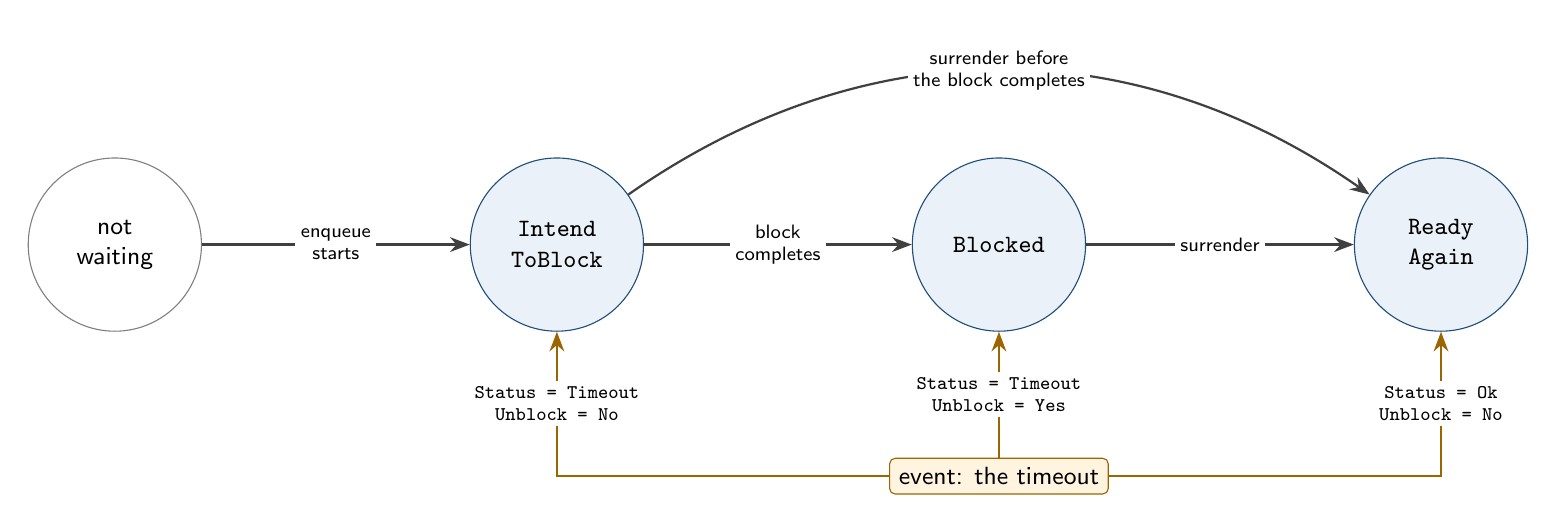
\begin{tikzpicture}[
    font=\small, node distance=34mm,
    st/.style={state, draw=ebblue, fill=boxfill, minimum size=22mm,
      align=center},
    pre/.style={st, fill=white, draw=gray},
    edge/.style={-{Stealth[length=2.5mm]}, thick, draw=flow},
    tmo/.style={-{Stealth[length=2.5mm]}, thick, draw=codeline},
    lbl/.style={font=\scriptsize, align=center, fill=white, inner sep=2pt}]
  \node[pre] (idle) {not\\waiting};
  \node[st, right=of idle] (itb) {\texttt{Intend}\\\texttt{ToBlock}};
  \node[st, right=of itb] (blk) {\texttt{Blocked}};
  \node[st, right=of blk] (rdy) {\texttt{Ready}\\\texttt{Again}};
  \draw[edge] (idle) -- node[lbl] {enqueue\\starts} (itb);
  \draw[edge] (itb) -- node[lbl] {block\\completes} (blk);
  \draw[edge] (blk) -- node[lbl] {surrender} (rdy);
  \draw[edge] (itb) to[bend left=35] node[lbl] {surrender before\\the block completes} (rdy);
  \node[draw=codeline, fill=codefill, rounded corners=2pt, align=center,
    below=16mm of blk] (to) {event: the timeout};
  \draw[tmo] (to) -- node[lbl] {\texttt{Status = Timeout}\\\texttt{Unblock = Yes}} (blk);
  \draw[tmo] (to) -| node[lbl, pos=0.75] {\texttt{Status = Timeout}\\\texttt{Unblock = No}} (itb);
  \draw[tmo] (to) -| node[lbl, pos=0.75] {\texttt{Status = Ok}\\\texttt{Unblock = No}} (rdy);
\end{tikzpicture}
\end{document}
